\chapter{Results}
\label{cha:res}
\label{res:Intro}
\todo{intro ch 6}

\section{Running the tests}
\label{res:RunningTests}
\label{res:Specs}
Although the specifications are not crucial since we did not do any speed benchmarking, it does give you, the reader, an idea of the performance. All tests where executed on an Ubuntu 20.04.5 LTS with 8GB RAM, an Intel core i5-3380M capable of 2.90GHz and a V-NAND SSD of 500GB 860 EVO Model MZ-76E500 through a SATA 3 connection. With each technique taking around a day to three days to run all nine thousand seed files once. Note that processing a seed once can mean that variants of that seed were run up to 100 times depending on the technique.

%time when faults are found?

\subsection{Preventing the same bug from occurring frequently}
%these tools often gave the same error again causing the new bug to be hidden, se choice to catch some of the more prevelent bugs, If some one wishes to rerun (parts) It is best to remove those exceptions in order to see the full output
While the techniques where running noticed that once a bug was found by any of our techniques that same bug would occur frequently but in a different seed, causing our resulting logs to be cluttered with duplicates bugs. We where aware that this could occur and we originally wanted to use deduplication as described in subsection \ref{inputReduction:Deduplication} to get rid of the duplicates. But after seeing 10 000 logs of the same bug, we changed from a reactive approach to a preventative approach. Once we noted a bug we tried to prevent it, for crashes this meant adding a try catch for the specific error. While, for wrongly (un)satisfiable we looked at special occurrences of keywords in constraint we knew caused bugs to then not log them. For example a bug we will discuss soon had a specific string of characters " == 0 == 0" making any problem wrongly unsatisfy. Being able to check the string of characters with knowing that it resulted in wrongly unsatisfiable  solutions made it for able for us to filter that bug as well. Luckily, with these restrictions on the output logs we were able to filter out most duplicate bugs, this is not an ideal solution but seems to work for now. The ideal solution would be that the fuzzer has knowledge of the already found bugs and reject them, techniques like these do exist but would bring us to far from the scope of the dissertation. Although, less efficient the techniques could be used for detecting an error fixing them and then rerunning for the next bug instead of adding exceptions.


\section{Results: found bugs}
\label{res:bugs}
In total we found 20 bugs, three of which were already submitted as an issue. Of those bugs some of them where easy fixes, some were a bit harder and required more time to solve. At the time of writing not al bugs are resolved (some are just reported days ago), but we look in anticipation how those will be solved. For now let's look at some of the most interesting bugs we found. 

\subsection{The four components of CPMpy}
\label{res:bugs:ComponentsCpMpy}
In order to do this we need some basics on how CPMpy works. CPMpy meanly exists out of four big parts a model part (everything to do with creating a model of a problem), a transformation part (everything to do with changing constraints), solver specific part transformations (everything to do with restrictions the solver puts on CPMpy) and then the solver themselves. This CPMpy has little to none controller over as can be seen in figure \ref{fig:4ComponentsOfCPMpy}. For now this is detailed enough, we leave the honor of a deeper analysis to the CPMpy-team to write about.

\begin{figure}
	\centering
	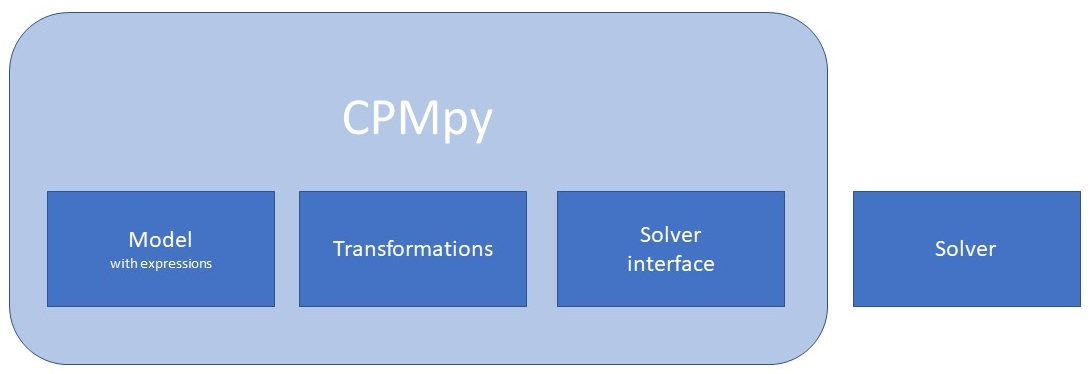
\includegraphics[width=1.0\textwidth]{images/4componentsOfCPMpy}
	\caption{Four main components of CPMpy}
	\label{fig:4ComponentsOfCPMpy}
\end{figure}
\todo{Why is this in my results?}

%We have shortly seen how a CPMpy looks like in listing \ref{lst:SendMoreMoneyCPMpy}, 
%where we create a model, add constraints to it and then to solve the model. Everything up to the solving part is controlled by CPMpy, once the "solve()" is called 

\subsection{Double Not}
\label{res:bug:DoubleNot}
The first bug we discovered was our "double not"-bug, a bug where we ask CPMpy to solve the constraints "X==3 and not(not(X==3))". Clearly this solution is trivial, set variable 'X' equal to 3 and the problem would be satisfied. However not all CPMpy solver did agreed with this, both OR-Tools and Gurobi said that this problem was unsatisfiable. 

This was due to a process within CPMpy responsible for creating a flat normal form. Not all solver used by CPMpy allow an arbitrary nesting of constraints as described by the documentation of CPMpy\footnote{\url{https://cpmpy.readthedocs.io/en/latest/behind_the_scenes.html}}. It is for that reason that CPMpy flattens the constraints to what they call 'flat normal forms' as the similar definition of SAT but with a disclaimer that this definition does not formally exists for CP languages to their knowledge, a statement which we agree with. With this flattened form CPMpy can directly call the solvers or do some solver specific transformations on the flattened constraints to then send it to the respective solver \cite{CPMpyGithub}. 

It was in this normalizing process that a comparison in a comparison was not handled (a 'not' gets translated to a comparison with zero "== 0"). Causing a disappearance of a single "not", which in turn resulted in "X==3 and not(X==3)" being send to OR-Tools and Gurobi. The other solvers, mainly MiniZinc's subsolvers, where not affected by this bug due to not using this normalizing process. Although, this normalizing process was subjected to unit tests, these tests contained an incorrect output causing the bug to remain under the radar. This bug was only caught using the modified STORM technique, due to its frequent use of adding "not"'s and "and"'s. But we believe it could have been caught in the differential testing if one of the seeds had a double not in its constraints or in the metamorphic testing if we had though of adding a relevant metamorphic transformation.


\subsection{Negation of Global functions}
\label{res:bug:NegatedGlobal}
A second bug related to the use of "not"'s were the crashes of the negated global functions. For example, "not(AllDifferent(argList))" would crash with a maximal recursion depth as the normalizing of a negated global function would be handled with adding a "== 0" to it, instead of decomposing the global function and negating that. The action of adding a "== 0" did not change the constraint and on the next normalizing of the left part of the comparison "global function == 0", the same would happen. The solution was as mentioned to decomposing the global function, which was suggested in de comments together with a commented out not-implemented warning. The entire function was labeled as work in progress, but the CPMpy-team expected it to work for this use case as they used it in their reification process. With a small but important caveat that this bug took a shortcut in de code, therefore exposing the bug. 

It was again due to the normalizing not being used for MiniZinc's subsolvers that the bug only occurred when using OR-Tools and Gurobi as solvers. This bug was quickly found by our modified STORM since it uses a significant number of "not"'s. It did not get found by our differential tests simply because no examples negated their global functions as such a negation is rarely useful. However, due to adding "!= 0" after constraints the metamorphic tests did find it as the bug as well.

\subsection{Power function of Gurobi}
\label{res:bug:Power}
Now that we have seen two bugs in the normalization part of CPMpy, which both fit in the transformations component of CPMpy, it is time to look at some solver specific transformations. 

\subsection{Wrong bound value Error}
\label{res:bug:WrongBounds}

neg values = crash
\subsection{Naming variables}
\label{res:bug:Naming+andImport}
var starting with '+' both import variable with same name
\subsection{Unsatisfiable Gurobi}
\label{res:bug:UnsatGurobu}

\subsection{Circuit of one}
\label{res:bug:Circuit}


\section{Classifications}
\subsection{Model, Transformation or Solver}

\begin{table}[]
	\centering
	\begin{tabular}{lll}
	BugNr & Bug description                                         & Place of the bug \\ \toprule
	142   & double not gives unsat                                  & Transformation   \\
	143   & negating global functions crashes                       & Transformation   \\
	145   & solvers lookup crashes                                  & Model            \\
	149   & negative lower bound in power function crashes          & Solver           \\
	150   & wrong bound gives causes a crash                        & Solver           \\
	152   & boolean variable does not support implies               & Model            \\
	153   & Gurobi does not run and gives the wrong nr of sol       & Solver           \\
	154   & JSON Decoder error                                      & Solver           \\
	155   & list has no shape                                       & solver           \\
	156   & MiniZinc returns zero causes a crash                    & Solver           \\
	157   & Circuit of one element crashes                          & Transformation   \\
	158   & Identical variable name can cause wrongly unsat         & Model            \\
	159   & Unhandled Gurobi exit status 9                          & Solver           \\
	161   & two separate references for the same variable           & Model            \\
	162   & CPMpy is looser with variable names than MiniZinc       & Solver           \\
	163   & Cyclic expression tee got generated                     & Model            \\
	164   & malloc() failure due to unset bounds                    & Transformation   \\
	165   & memory violation segmentation fault                     & Transformation   \\
	168   & unsatisfiable Gurobi                                    & Transformation   \\
	170   & unsatisfiable due to flattening                         & Transformation   \\ \bottomrule        
	\end{tabular}
	\caption{A table with the correct layout.}
	\label{tab:bug:place}
\end{table}

Tabel + bespreken
\subsection{crash or wrongly (un)sat}
\begin{table}[]
	\centering
	\begin{tabular}{lll}
		BugNr & Bug description                                           & Type of fault   \\ \toprule
		142   & double not gives unsat                                    & wrongly unsat   \\
		143   & negating global functions crashes                         & crash           \\
		145   & solvers lookup crashes                                    & crash           \\
		149   & negative lower bound in power function crashes            & crash           \\
		150   & wrong bound gives causes a crash                          & crash           \\
		152   & boolean variable does not support implies                 & crash           \\
		153   & Gurobi does not run and gives the wrong nr of sol         & did not run     \\
		154   & JSON Decoder error                                        & crash           \\
		155   & list has no shape                                         & crash           \\
		156   & MiniZinc returns zero causes a crash                      & crash           \\
		157   & Circuit of one element crashes                            & crash           \\
		158   & Identical variable name can cause wrongly unsat           & wrongly unsat   \\
		159   & Unhandled Gurobi exit status 9                            & crash           \\
		161   & two separate references for the same variable             & wrongly unsat   \\
		162   & CPMpy is looser with variable names than MiniZinc         & crash           \\
		163   & Cyclic expression tee got generated                       & crash           \\
		164   & malloc() failure due to unset bounds                      & crash           \\
		165   & memory violation segmentation fault                       & crash           \\
		168   & wrongly unsatisfiable Gurobi                              & wrongly unsat   \\
		170   & wrongly (un)satisfiable due to flattening                 & wrongly (un)sat \\ \bottomrule
	\end{tabular}
	\caption{A table with the correct layout.}
	\label{tab:bug:fault}
\end{table}

Tabel + bespreken
\subsection{which solver}
\begin{table}[]
	\centering
	\begin{tabular}{lll}
		BugNr & Bug description                                           & Which solver caused it?\\ \toprule
		142   & double not gives unsat                                    & OR-Tools and Gurobi                            \\
		143   & negating global functions crashes                         & OR-Tools and Gurobi                            \\
		145   & solvers lookup crashes                                    & solver independent                             \\
		149   & negative lower bound in power function crashes            & MiniZinc's subsolver Gurobi                    \\
		150   & wrong bound gives causes a crash                          & all pysat subsolvers                           \\
		152   & boolean variable does not support implies                 & solver independent                             \\
		153   & Gurobi does not run and gives the wrong nr of sol         & Gurobi                                         \\
		154   & JSON Decoder error                                        & MiniZinc's subsolver osicbc                    \\
		155   & list has no shape                                         & Gurobi                                         \\
		156   & MiniZinc returns zero causes a crash                      & multiple MiniZinc subsolvers                   \\
		157   & Circuit of one element crashes                            & solver independent                             \\
		158   & Identical variable name can cause wrongly unsat           & solver independent                             \\
		159   & Unhandled Gurobi exit status 9                            & Gurobi                                         \\
		161   & two separate references for the same variable             & solver independent                             \\
		162   & CPMpy is looser with variable names than MiniZinc         & all MiniZinc subsolvers                        \\
		163   & Cyclic expression tee got generated                       & solver independent                             \\
		164   & malloc() failure due to unset bounds                      & multiple MiniZinc subsolvers                   \\
		165   & memory violation segmentation fault                       & multiple MiniZinc subsolvers                   \\
		168   & wrongly unsatisfiable Gurobi                              & Gurobi                                         \\
		170   & wrongly (un)satisfiable due to flattening                 & OR-Tools and Gurobi                            \\ \bottomrule
	\end{tabular}
	\caption{A table with the correct layout.}
	\label{tab:bug:Solver}
\end{table}

Tabel + bespreken
\subsection{which technique could find it}
Tabel + bespreken
\begin{table}[]
	\centering
	\begin{tabular}{lllll}
		BugNr & Bug description                                           & \multicolumn{3}{l}{Found by which technique} \\ \toprule
		142   & double not gives unsat                                    & storm          &              &              \\
		143   & negating global functions crashes                         & storm          &              & meta         \\
		145   & solvers lookup crashes                                    &                & diff         &              \\
		149   & negative lower bound in power function crashes            & storm          & diff         &              \\
		150   & wrong bound gives causes a crash                          &                & diff         &              \\
		152   & boolean variable does not support implies                 &                & diff         & meta         \\
		153   & Gurobi does not run and gives the wrong nr of sol         &                & diff         &              \\
		154   & JSON Decoder error                                        & storm          & diff         & meta         \\
		155   & list has no shape                                         & storm          & diff         & meta         \\
		156   & MiniZinc returns zero causes a crash                      & storm          & diff         & meta         \\
		157   & Circuit of one element crashes                            &                &              & meta         \\
		158   & Identical variable name can cause wrongly unsat           &                &              & meta         \\
		159   & Unhandled Gurobi exit status 9                            & storm          & diff         &              \\
		161   & two separate references for the same variable             & storm          &              & meta         \\
		162   & CPMpy is looser with variable names than MiniZinc         &                &              & meta         \\
		163   & Cyclic expression tee got generated                       &                &              & meta         \\
		164   & malloc() failure due to unset bounds                      &                &              & meta         \\
		165   & memory violation segmentation fault                       &                & diff         & meta         \\
		168   & wrongly unsatisfiable Gurobi                              & storm          & diff         & meta         \\
		170   & wrongly (un)satisfiable due to flattening                 & storm          &              & meta         \\ \bottomrule
	\end{tabular}
	\caption{A table with the correct layout.}
	\label{tab:bug:Technique}
\end{table}


\section{Reception to the bugs}
they where happy :p
The double Not bug \ref{res:bug:DoubleNot} was called a serious bug and a great find. % https://github.com/CPMpy/cpmpy/issues/142#issuecomment-1312530262

\ref{res:bug:NegatedGlobal}
unexpected bug as the code is used often in reification, but this used a shortcut
% https://github.com/CPMpy/cpmpy/issues/143#issuecomment-1312522873


\section{STORM}
Techniques are best applied during development, since the modified storm of to often detects the already fond bugs

%problems limited by global fucntions of used seeds (somewhat fine),
%only 'and' and 'not' combinations Just like STORM

~(~(True))
~(global function)
\section{Differential testing}
solverlookup()  was during development = manual testing, 

\section{Metamorphic testing}
did not find ~(~()) simly because we dind't think to check it specificly, we did check ~=0
all checks ? + combo-able

\section{YinYang}


\section{unsat}
due to the way of importing the file a lot of edge problems become sat or unsat

\section{woringly sat}
meta unsat minizinc 0
to shirk this we used the fact that ortools+gurobi (probably) gave the correct solution, this being unsat and taking the mus from that


\subsection{finding mus}
combination of their tool, but when we got errors from the different way of loading, We used my tool en then theirs. general combinations were done got get a minimal. 
my tool incapable of pure MUS





\section{Conclusion}
\todo{Conclusion}
The final section of the chapter gives an overview of the important results
of this chapter. This implies that the introductory chapter and the
concluding chapter don't need a conclusion.

%%% Local Variables: 
%%% mode: latex
%%% TeX-master: "thesis"
%%% End: 
